\section{Coordinate Systems and Vector-Valued Functions}

\subsection{Coordinate Systems in 3D Space}

Specifying a point or giving directions in space can be accomplished in multiple ways:
\begin{itemize}
    \item Giving a direction and a distance.
    \item Using Cartesian coordinates $(d_1, d_2, d_3) = (x, y, z)$.
    \item Specifying an angle relative to a reference axis along with a magnitude.
    \item Referencing a relative landmark.
    \item Using geographic coordinates like latitude and longitude.
\end{itemize}

\subsubsection{Polar Coordinates (2D)}
In the $xy$-plane, a point is specified by its radial distance $r$ from the origin and an angle $\theta$ relative to the positive $x$-axis: $(r, \theta)$.

\[
r = \sqrt{x^2 + y^2} \quad (r \ge 0)
\]

While $\theta = \arctan\left(\frac{y}{x}\right)$ is commonly used, it is undefined when $x = 0$. The foundational algebraic transformation between systems is given by:
\begin{align*}
x &= r\cos\theta \\
y &= r\sin\theta
\end{align*}


\subsubsection{Cylindrical Coordinates}
Cylindrical coordinates $(r, \theta, z)$ extend polar coordinates into 3D space by preserving the standard Cartesian $z$-axis:
\begin{align*}
x &= r\cos\theta \\
y &= r\sin\theta \\
z &= z
\end{align*}

\subsubsection{Spherical Coordinates}
Spherical coordinates are represented as $(\rho, \theta, \phi)$, where $\rho$ is the distance from the origin, $\theta$ is the azimuthal angle in the $xy$-plane, and $\phi$ is the polar angle measured down from the positive $z$-axis.

\begin{align*}
x &= \rho\sin\phi\cos\theta \\
y &= \rho\sin\phi\sin\theta \\
z &= \rho\cos\phi
\end{align*}

The standard domain boundaries are:
\begin{align*}
\rho &\ge 0 \\
0 &\le \theta < 2\pi \\
0 &\le \phi \le \pi
\end{align*}

\begin{center}
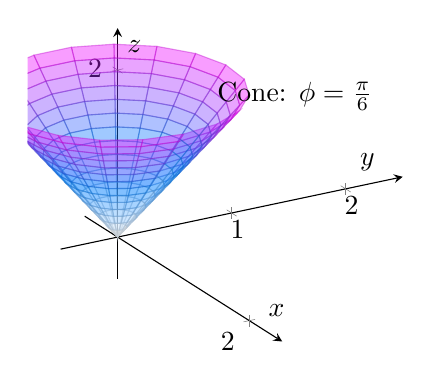
\begin{tikzpicture}
\begin{axis}[
    view={60}{30},
    axis lines=center,
    xlabel={$x$}, ylabel={$y$}, zlabel={$z$},
    xmin=-0.5, xmax=2.5, ymin=-0.5, ymax=2.5, zmin=-0.5, zmax=2.5
]
    % Cone for phi = pi/6
    \addplot3[surf, domain=0:2, domain y=0:360, samples=15, samples y=20, variable=\r, variable y=\t, opacity=0.4, colormap/cool]
        ({r*sin(30)*cos(t)}, {r*sin(30)*sin(t)}, {r*cos(30)});
    \node[anchor=south west] at (axis cs: 0.5,0.5,1.5) {Cone: $\phi = \frac{\pi}{6}$};
\end{axis}
\end{tikzpicture}
\end{center}

\subsection{Coordinate System Transformations}

\begin{problem}{Conversion Between Coordinate Systems}{conversion_between_coordinate_systems}
Convert the surface equation $x^2 + \dfrac{y^2}{a^2} = z^2$ into cylindrical and spherical coordinates.
\end{problem}

\begin{sol}
\textbf{Cylindrical Coordinates:} \\
Substituting $x = r\cos\theta$, $y = r\sin\theta$, and $z = z$ into the original equation yields:
\begin{align*}
(r\cos\theta)^2 + \frac{(r\sin\theta)^2}{a^2} &= z^2 \\
r^2\cos^2\theta + \frac{r^2\sin^2\theta}{a^2} &= z^2 \\
r^2\left(\cos^2\theta + \frac{\sin^2\theta}{a^2}\right) &= z^2
\end{align*}

\textbf{Spherical Coordinates:} \\
Substituting $x = \rho\sin\phi\cos\theta$, $y = \rho\sin\phi\sin\theta$, and $z = \rho\cos\phi$ into the original equation yields:
\begin{align*}
(\rho\sin\phi\cos\theta)^2 + \frac{(\rho\sin\phi\sin\theta)^2}{a^2} &= (\rho\cos\phi)^2 \\
\rho^2\sin^2\phi\cos^2\theta + \frac{\rho^2\sin^2\phi\sin^2\theta}{a^2} &= \rho^2\cos^2\phi \\
\rho^2\sin^2\phi\left(\cos^2\theta + \frac{\sin^2\theta}{a^2}\right) &= \rho^2\cos^2\phi
\end{align*}
Assuming $\rho \neq 0$, we divide both sides by $\rho^2$:
\begin{align*}
\sin^2\phi\left(\cos^2\theta + \frac{\sin^2\theta}{a^2}\right) &= \cos^2\phi \\
\cos^2\theta + \frac{\sin^2\theta}{a^2} &= \frac{\cos^2\phi}{\sin^2\phi} \\
\cos^2\theta + \frac{\sin^2\theta}{a^2} &= \cot^2\phi
\end{align*}
\end{sol}

\subsection{Vector-Valued Functions}

\begin{definition}{Vector-Valued Functions}{vector_value_functions}
A vector-valued function maps one or more real parameters to a space vector:
\[
\vv{r}(t) = \ang{x(t), y(t), z(t)}, \quad \vv{r}: I \rightarrow \mathbb{R}^3
\]
where $I \subseteq \mathbb{R}$ is an interval. This traces out a spatial curve parametrized by $t$.
\end{definition}

\begin{example}
Consider the vector function $\vv{r}(t) = \ang{\cos t, \sin t, 1}$ for $0 \le t < 2\pi$. This describes a unit circle in 3D space elevated to the horizontal plane $z = 1$.

\begin{center}
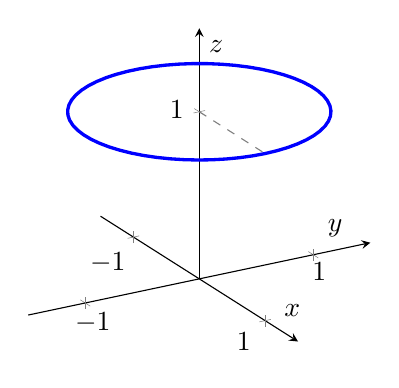
\begin{tikzpicture}
\begin{axis}[
    view={60}{30},
    axis lines=center,
    xlabel={$x$}, ylabel={$y$}, zlabel={$z$},
    xmin=-1.5, xmax=1.5, ymin=-1.5, ymax=1.5, zmin=0, zmax=1.5
]
    \addplot3[domain=0:360, samples=60, samples y=0, line width=1.2pt, blue]
        ({cos(x)}, {sin(x)}, {1});
    \draw[dashed, gray] (axis cs: 0,0,1) -- (axis cs: 1,0,1);
\end{axis}
\end{tikzpicture}
\end{center}
\end{example}

\begin{problem}{Finding Collisions and Intersections}{finding_collisions}
Let $\vv{r}_1(t) = \ang{t^2 + \dfrac{t}{2}, t - t^3}$ and $\vv{r}_2(t) = \ang{t, t^2}$. Find all collision points and structural intersections between the curves.
\end{problem}

\begin{sol}
\textbf{1. Collision Points (Same location at same time $t$):} \\
Setting $\vv{r}_1(t) = \vv{r}_2(t)$ gives:
\begin{align*}
\ang{t^2 + \dfrac{t}{2}, t - t^3} &= \ang{t, t^2}
\end{align*}
Equating the individual components gives the system:
\begin{align*}
t^2 + \frac{t}{2} &= t \\
t - t^3 &= t^2
\end{align*}
Solving the first equation for $t$:
\begin{align*}
t^2 + \frac{t}{2} - t &= 0 \\
t^2 - \frac{t}{2} &= 0 \\
t\left(t - \frac{1}{2}\right) &= 0 \implies t = 0 \quad \text{or} \quad t = \frac{1}{2}
\end{align*}
Now, we verify both parameters in the second component equation $t - t^3 = t^2$:
\begin{align*}
\text{For } t = 0: \quad 0 - (0)^3 &= (0)^2 \implies 0 = 0 \quad \text{(Valid)} \\
\text{For } t = \frac{1}{2}: \quad \frac{1}{2} - \left(\frac{1}{2}\right)^3 &= \frac{1}{2} - \frac{1}{8} = \frac{3}{8} \\
\left(\frac{1}{2}\right)^2 &= \frac{1}{4} = \frac{2}{8} \neq \frac{3}{8} \quad \text{(Invalid)}
\end{align*}
Therefore, $t = 0$ is the only valid collision time. Evaluating $\vv{r}_1(0)$:
\begin{align*}
\vv{r}_1(0) &= \ang{0^2 + \frac{0}{2}, 0 - 0^3} = \ang{0, 0}
\end{align*}
The collision point is $(0, 0)$.

\textbf{2. Intersection Points (Same location at potentially different times $t$ and $s$):} \\
Setting $\vv{r}_1(t) = \vv{r}_2(s)$ gives:
\begin{align*}
\ang{t^2 + \frac{t}{2}, t - t^3} &= \ang{s, s^2}
\end{align*}
Equating components yields:
\begin{align*}
s &= t^2 + \frac{t}{2} \tag{1} \\
t - t^3 &= s^2 \tag{2}
\end{align*}
Substituting equation (1) into equation (2):
\begin{align*}
t - t^3 &= \left(t^2 + \frac{t}{2}\right)^2 \\
t - t^3 &= t^4 + t^3 + \frac{t^2}{4} \\
0 &= t^4 + 2t^3 + \frac{t^2}{4} - t \\
0 &= t\left(t^3 + 2t^2 + \frac{t}{4} - 1\right)
\end{align*}
Setting each factor to zero:
\begin{align*}
t = 0 & \implies s = 0^2 + \frac{0}{2} = 0 \\
&\implies \text{Intersection point } (0, 0) \\
t^3 + 2t^2 + \frac{t}{4} - 1 = 0 & \implies t \approx 0.576
\end{align*}
Solving for $s$ when $t \approx 0.576$:
\begin{align*}
s &= (0.576)^2 + \frac{0.576}{2} \\
s &\approx 0.332 + 0.288 \approx 0.620
\end{align*}
Evaluating the spatial coordinates using $\vv{r}_2(s)$:
\begin{align*}
x &= s \approx 0.620 \\
y &= s^2 \approx (0.620)^2 \approx 0.384
\end{align*}
Hence, the two spatial intersection points are $(0, 0)$ and $(0.620, 0.384)$.
\end{sol}

\subsection{Gallery of Parametric Space Curves}

Below are standard parametric 3D space curves used in multivariable trajectory analysis:

\begin{center}
\begin{minipage}{0.32\textwidth}
\centering
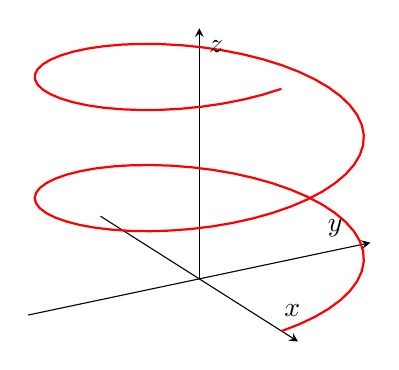
\begin{tikzpicture}
\begin{axis}[
    view={60}{30},
    axis lines=center,
    xlabel={$x$}, ylabel={$y$}, zlabel={$z$},
    xmin=-1.2, xmax=1.2, ymin=-1.2, ymax=1.2, zmin=0, zmax=13,
    ticks=none
]
    \addplot3[domain=0:4*pi, samples=100, samples y=0, thick, red]
        ({cos(deg(x))}, {sin(deg(x))}, {x});
\end{axis}
\end{tikzpicture}
\\[0.5em]
$\vv{r}(t) = \ang{\cos t, \sin t, t}$
\end{minipage}
\hfill
\begin{minipage}{0.32\textwidth}
\centering
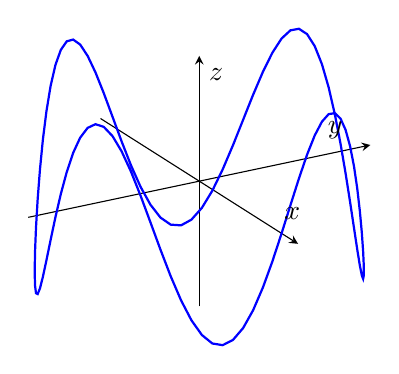
\begin{tikzpicture}
\begin{axis}[
    view={60}{30},
    axis lines=center,
    xlabel={$x$}, ylabel={$y$}, zlabel={$z$},
    xmin=-1.2, xmax=1.2, ymin=-1.2, ymax=1.2, zmin=-1.2, zmax=1.2,
    ticks=none
]
    \addplot3[domain=0:2*pi, samples=100, samples y=0, thick, blue]
        ({cos(deg(x))}, {sin(deg(x))}, {sin(4*deg(x))});
\end{axis}
\end{tikzpicture}
\\[0.5em]
$\vv{r}(s) = \ang{\cos s, \sin s, \sin(4s)}$
\end{minipage}
\hfill
\begin{minipage}{0.32\textwidth}
\centering
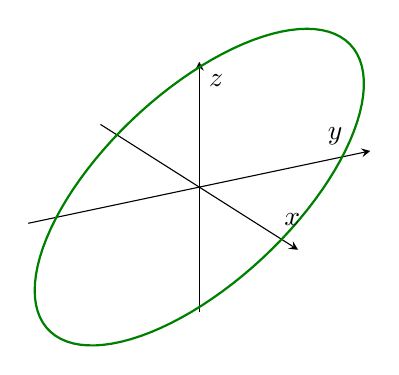
\begin{tikzpicture}
\begin{axis}[
    view={60}{30},
    axis lines=center,
    xlabel={$x$}, ylabel={$y$}, zlabel={$z$},
    xmin=-1.2, xmax=1.2, ymin=-1.2, ymax=1.2, zmin=-4.2, zmax=4.2,
    ticks=none
]
    \addplot3[domain=0:2*pi, samples=100, samples y=0, thick, green!50!black]
        ({cos(deg(x))}, {sin(deg(x))}, {4*sin(deg(x))});
\end{axis}
\end{tikzpicture}
\\[0.5em]
$\vv{r}(t) = \ang{\cos t, \sin t, 4\sin t}$
\end{minipage}
\end{center}